\subsection{Determining the radiation power at the trap region}
\label{subsec:rot:power}

The radiation power reaching the trap region is determined by the geometry of the trap 
and the intensity profile of the laser beam. In this section, we discuss the
estimation of the radiation power reaching the trap region for a given laser beam
frequency and intensity profile.

\begin{figure}[!htb]
    \centering
    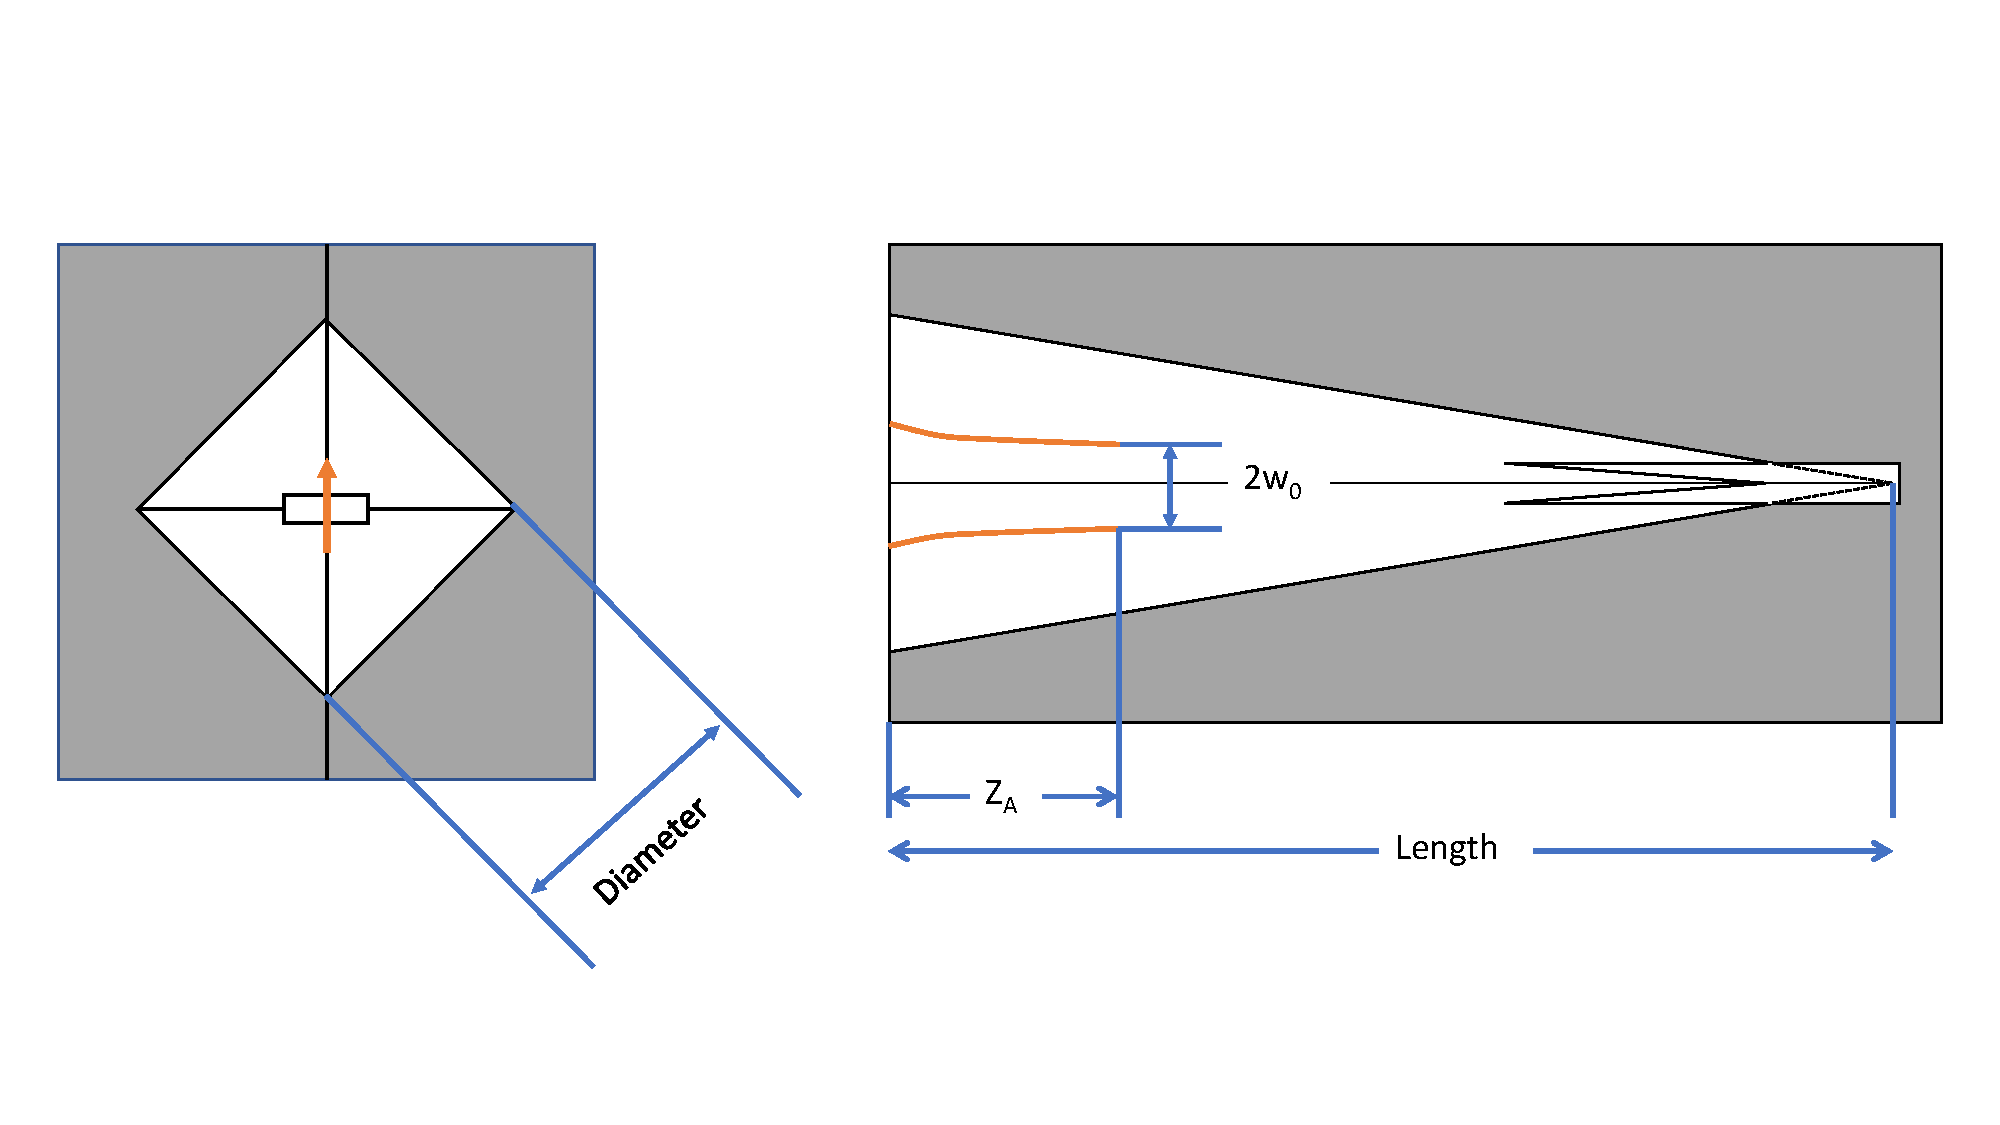
\includegraphics[width=0.9\textwidth]{figures/measurements/power-curve-453GHz/THz feed horn.pdf}
    \caption{Schematics of the nominal feed horn antenna are shown. Z$_A$ is defined as the location of the beam waist radius (w$_0$) with respect to the horn aperture. The upward arrow (orange solid line) indicates the polarisation direction of the electric field.}
    \label{fig:feed-horn}
\end{figure}

The feed horn antenna's electric field radiation emitted/propagated is shown in
Figure \ref{fig:feed-horn}. The propagation of the emitted Gaussian beam radius
($w(z)$) from a horn antenna is given by:

\begin{figure}[!htb]
    \centering
    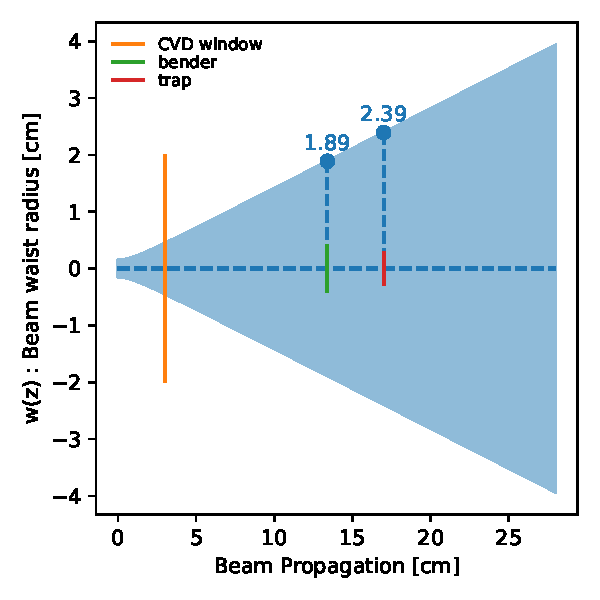
\includegraphics[scale=0.7]{figures/measurements/power-curve-453GHz/beam_propagation.pdf}
    \caption{Gaussian beam (for a frequency of $\nu=453$ GHz) propagation from a beam waist radius of 0.15 cm produced from diagonal feed horn antenna. The solid lines - orange and green indicate the position of the FELion instrument entrance window (CVD diamond window, 3 cm from antenna, 2 cm aperture radius) and bender (10.4 cm from window, 0.43 cm aperture radius), 22-pole ion-trap (14 cm from window, 0.3 cm aperture radius), respectively.}
    \label{fig:power-curve:beam-propagation}
\end{figure}

\begin{equation}
    w(z) = w_0 * \sqrt{1 + \left( \frac{z}{Z_R} \right) ^2}
    \label{eqn:beam-propagation}
\end{equation}
where $Z_R$ is the Rayleigh length (or Rayleigh range) for Gaussian beams.

$Z_R$  is determined by the waist radius $w_0$ and the wavelength ($\lambda$) as shown below:

\[Z_R = \frac{\pi \cdot w_0^2}{\lambda}\]

The Gaussian beam propagation simulation for a frequency $\Delta \nu = 453$ GHz is
shown in Figure \ref{fig:power-curve:beam-propagation}, 
using a diagonal horn antenna (VDI waveguide band WM-570) of length, 
aperture diameter and beam waist radius of 36, 3.6 and 1.5 mm, respectively

\begin{figure}[!htb]
    \centering
    \begin{subfigure}{0.49\textwidth}
        \centering
        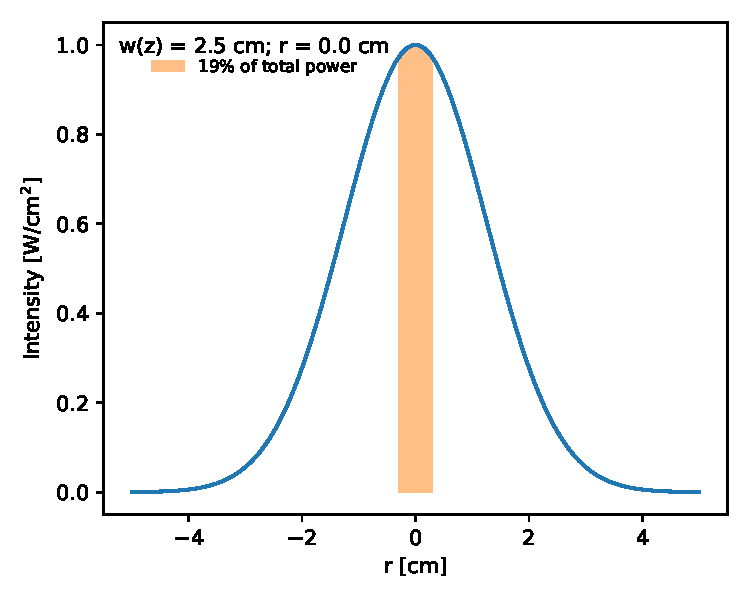
\includegraphics[width=1\textwidth]{figures/measurements/power-curve-453GHz/beam_propagation_power_curve_w0-2.50_offset-0.00_dia-0.60.pdf}
        \caption{}
        \label{fig:power-curve:beam-propagation-power:at0}
    \end{subfigure}
    \hfill
    \begin{subfigure}{0.49\textwidth}
        \centering
        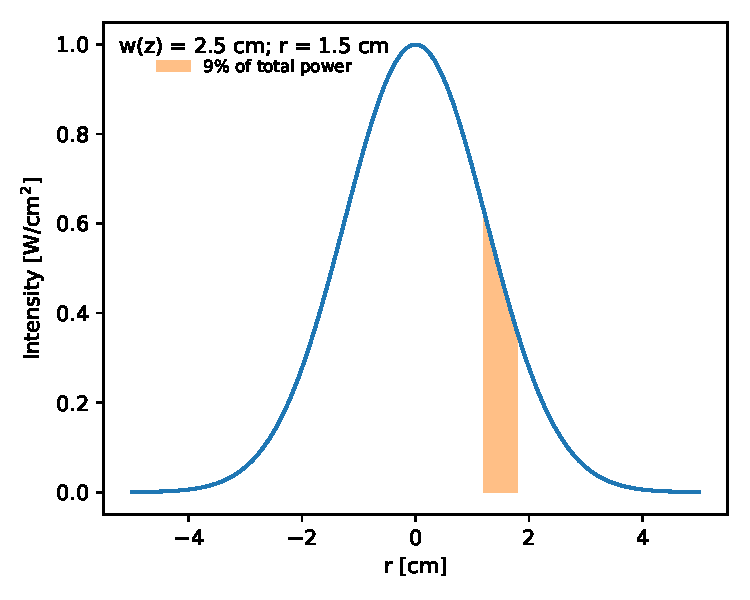
\includegraphics[width=1\textwidth]{figures/measurements/power-curve-453GHz/beam_propagation_power_curve_w0-2.50_offset-1.50_dia-0.60.pdf}
        \caption{}
        \label{fig:power-curve:beam-propagation-power:offset}
    \end{subfigure}
    \caption{The radiation intensity profile distribution is shown in the blue line. The shaded orange region indicates the fraction of output power at a 0.3 cm beam radius, i.e., inside trap region as shown in Figure \ref{fig:power-curve:beam-propagation}. The position of the orange region \emph{w.r.t} the x-axis represents the part of the propagating Gaussian beam reaching the trap region when (a): aligned and (b): 1.5 cm offset \emph{w.r.t} beam centre.}
    \label{fig:power-curve:beam-propagation-power}
\end{figure}


As the Gaussian laser beam propagates, the waist radius increases in size and
the corresponding intensity profile of the electric field is given by:

\begin{equation}
    \begin{split}
        I(r) & = I_0 \cdot exp \left[ -2 \left (\frac{r}{w(z)}\right ) ^2\right] \\
        & = \frac{2P}{\pi w(z)^2}
        \cdot exp \left[ -2 \left (\frac{r}{w(z)}\right ) ^2\right]
    \end{split}
    \label{eqn:beam-propagation:intensity}
\end{equation}

where $I_0$ is the peak irradiance at the centre of the beam, r is the radial
distance away from the propagation axis, w(z) is the radius of the laser beam
where the irradiance is 1/e$^2$ (13.5\%) of $I_0$, z is the distance propagated
from the plane where the wavefront is flat, and P is the total power of the
beam.\\

Figure \ref{fig:power-curve:beam-propagation-power} shows the intensity profile
using Eq. \ref{eqn:beam-propagation:intensity}, when the beam waist radius,
$w(z)=2.5$ cm, is at the trap entrance (see Figure
\ref{fig:power-curve:beam-propagation}). Since the ion-trap aperture diameter
is 0.3 cm which is much narrower compared to the incoming beam radius (2.5 cm),
one needs to consider an offset for the Gaussian beam centre reaching the trap
centre. Therefore, the figure \ref{eqn:beam-propagation:intensity} also
features the orange marked region, which indicates the actual power estimated
to reach the trap depending on its alignment, $r(z)$, \emph{w.r.t} the
propagating Gaussian beam centre, $r_0(z)$. If we assume that in our
experiment, $r(z)=0-1.5$ cm, then the final radiation power reaching the trap,
for $\Delta \nu=453$ GHz frequency is 9-19 \% of the peak power (250 $\mu$W),
i.e., $35(12)\ \mu$W.

% However, one can 100 \% focus the beam into the trap using a combination of radiation source and optics. The optics design and details are discussed in Section \ref{subsec:THz-optics}.